%%%%%%%%%%%%%%%%%%%%%%%%%%%%%%%%%%%%%%%%%%%%%%%%%%%%%%%%%%%%
\section{Pressure vessel} \label{sec:PressureVessel}
%%%
The pressure vessel of NEXT-DEMO, shown in figure~\ref{fig:Vessel}, is a stainless-steel (grade 304L) cylindrical shell, 3 mm thick, 30 cm diameter and 60 cm length, welded to CF flanges on both ends. The two end-caps are 3-cm thick plates with standard CF knife-edge flanges. Flat copper gaskets are used as sealing. The vessel was certified to 10 bar operational pressure. It was designed at IFIC and built by Trinos Vacuum Systems, a local manufacturer. Additional improvements --- including the support structure and a rail system to open and move the end-caps --- have been made using the mechanical workshop at IFIC.

%%%%%%%%%%
\begin{figure}
\centering
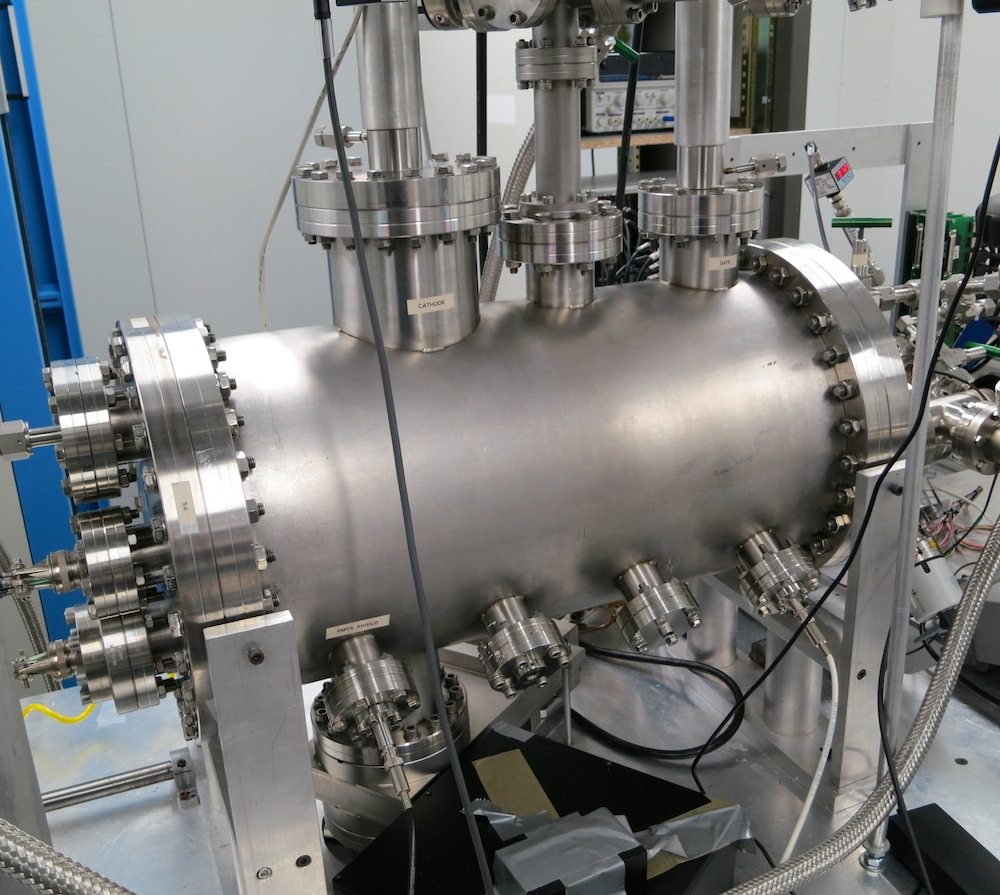
\includegraphics[scale=0.9]{img/VesselCloseup.jpg}
\caption{The pressure vessel of NEXT-DEMO.} \label{fig:Vessel}
\end{figure}
%%%%%%%%%%

The side of the chamber includes 8 CF40 half-nipples. One set of 4 is located in the horizontal plane while the other is displaced towards the underside with respect to the first set by $60^\circ$. These contain radioactive source ports used for calibration of the TPC. The ports are made by welding a 0.5 mm thick blank SS plate onto a 12 mm OD pipe on a CF40 liquid feedthrough. On top of the vessel and along the vertical plane there are three additional half-nipples (CF130, CF67 and CF80) used for high-voltage input and connection to a mass spectrometer (through a leak valve). On the opposite side, at the bottom, a CF100 port connects the pressure vessel to the vacuum pumping system. A guillotine valve closes this connection when the vessel is under pressure. The end-caps include several CF ports for the connections to the gas recirculation loop and for the feedthroughs (power and signal) of the PMT planes.
